% !TEX root = ../../../main.tex
% 来源：高中物理甲种本·第三册（电磁·光学·近代物理）
% 章节：光的反射和折射 / 透镜成像作图法
% 原始文件：5.tex，行 1590-1613
% 类型：tikz
% ---
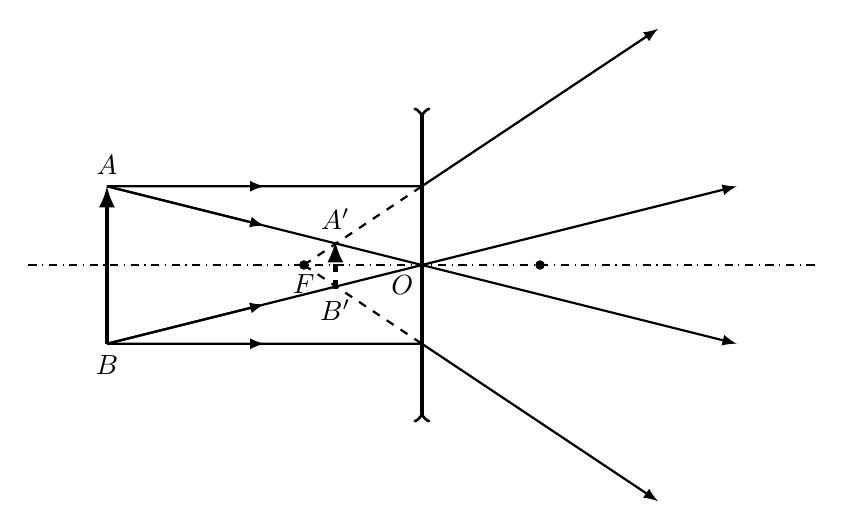
\begin{tikzpicture}
    \draw[>-<, very thick ] (0,2)--(0,-2);
    \draw[dashdotted](-5,0)--(5,0);
    \node at (-1.5,0)[below]{$F$};\node at (-.25,-.25){$O$};
    \draw [fill=black] (-1.5,0) circle (1.5pt);
    \draw [fill=black] (1.5,0) circle (1.5pt);

    \draw [->, ultra thick, >=latex] (-4,-1)node[below]{$B$}--(-4,1)node[above]{$A$};

    \draw [->,  thick, >=latex](-4,1)--(0,1)--(3,3); 
    \draw [->,  thick, >=latex](-4,-1)--(0,-1)--(3,-3); 
    \draw [thick, dashed](-1.5,0)--(0,-1);
    \draw [thick, dashed](-1.5,0)--(0,1);
\draw[->,  thick, >=latex] (-4,1)--(0,0)--(4,-1);
\draw[->,  thick, >=latex] (-4,-1)--(0,0)--(4,1);
\draw[->,  thick, >=latex] (-4,1)--(-2,0.5);
\draw[->,  thick, >=latex] (-4,-1)--(-2,-.5);
\draw [->,  thick, >=latex](-4,1)--(-2,1);
\draw [->,  thick, >=latex](-4,-1)--(-2,-1);
\draw [->, ultra thick, >=latex, dashed ] (-1.1,-.3)node[below]{$B'$}--(-1.1,.3)node[above]{$A'$};



\end{tikzpicture}
